\chapter{Interaktion zwischen Komponenten}

\section{Interaktion von App Komponenten}
 
\begin{figure}[H]
\centering
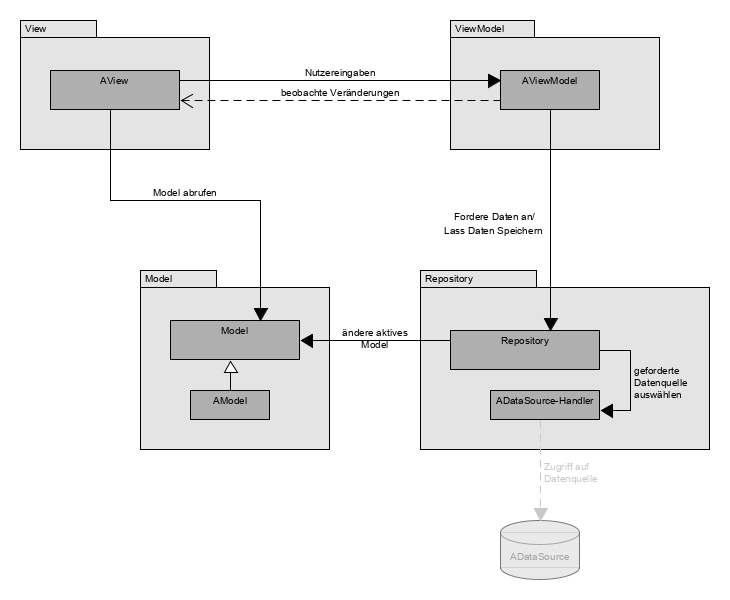
\includegraphics[width=0.7\textwidth]{pics/appComponentInteractions.png}%
\caption{Interaktion der App-Komponenten}%
\label{appcomp}%
\end{figure}


%AppComponentInteractions UML hier einfügen
Diagramm \ref{appcomp} beschreibt die Interaktion zwischen den einzelnen App-Komponenten etwas spezifischer als im vorigen Kapitel.
Zu beachten ist dabei, dass die angezeigten Komponenten "`AView"', "`AViewModel"', "`AModel"' und "`DataSource"' nur beispielhafte Instanzen darstellen. Jedes der ihnen zugrundeliegenden Pakete kann noch weitere Instanzen enthalten, die hier zur Anschaulichkeit vernachlässigt wurden.
Die Interaktion der App-Komponenten funktioniert folgendermaßen:
Ändert ein Nutzer Daten über die Benutzeroberfläche, so wird in der derzeit aktiven View-Komponente ("`AView"') eine Änderung vom zugehörigen ViewModel ("`AViewModel) registriert. Dieses gibt an das Repository durch, welche Daten geladen oder verändert werden müssen. Das Repository fordert daraufhin entweder Daten vom Server an, bzw. veranlasst eine Aktualisierung der Serverdaten, oder es holt, bzw. aktualisiert die Daten aus der lokalen SQLite-Datenbank ("`ADataSource"'). Außerdem aktualisiert das Repository das momentan aktive Model ("`AModel"') und gibt diesem die gerade geladenen oder aktualisierten Daten. Dadurch können neue Daten in der View angezeigt werden.

\section{Interaktion von Serverkomponenten}

In dem API Package des Servers(siehe Kapitel 4.2) befindet sich eine Menge an Interfaces, die angeben, wie man vom Client auf die API zugreifen kann. Diese Interfaces werden von den Controller-Klassen implementiert, insbesondere wird jede API-Klasse von einem zugehörigen Controller implementiert. 
Die Controller bearbeiten die Anfragen, die von den App-Klassen an den Server gestellt werden. Dabei rufen sie Serviceklassen auf, welche dann auf sogenannte "`Data Access Objekte"' (DAOs) zugreifen, um entweder Daten zu laden oder Daten zu speichern. Die Serviceklassen geben, wenn Daten angefragt wurden, die geladenen Daten an die Controller zurück und durch die Controller werden dann die Daten an den Client geschickt.
Bevor ein Client Daten anfragen oder senden kann, muss dieser erst Authentifiziert werden. Dazu wird ein JSON-Web-Authentification-Token, welcher bei der Anfrage mitgesendet wird, durch die Firebaselibrary überprüft.


\section{App- und Server-Kommunikation}

\begin{figure}[H]
\centering
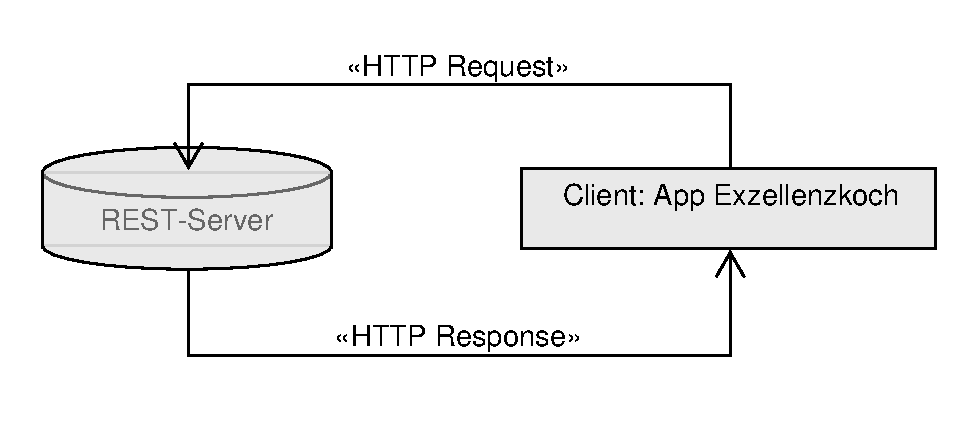
\includegraphics[width=0.7\textwidth]{pics/ServerAppRESTInteraction.pdf}%
\caption{Server-AppkKommunikation über REST}%
\label{rest}%
\end{figure}

Der Server bietet eine REST-Schnittstelle. Über diesen kommunizieren App und Server miteinander.
Hierbei wird das Request-Response Verfahren verwendet, wie in Abbildung \ref{rest} vereinfacht gezeigt. Der Client schickt eine Anfrage an den Server. Eine Anfrage verwendet das HTTP-Protokoll. Entweder wird eine GET-, POST-, PUT- oder DELETE-Anfrage gesendet. Der Server bearbeitet die Anfrage und gibt eine Antwort zurück. Die Daten werden als JSON-Dateien versendet. Die Verbindung zwischen Client und Server besteht, solange die Anfrage und Antwort durchgeführt, oder eine Zeitbegrenzung überschritten wird. 
Statt dass die App ganze Entity-Objekte an den Server sendet, werden diese in "`Data Transfer Objects"' (DTOs) abstrahiert. Die DTOs sind so aufgebaut, dass sie auf die Server-Datenbank Tabellen gemapped werden können. Mehr zum Aufbau der DTOs ist in Kapitel \ref{kapdtos} zu finden.
%https://www.itwissen.info/Request-Response-Verfahren-request-response-method.html

%\section{Interaktion der Appkomponenten} 
%Grafik \ref{rrr} zeigt ein einen Überblick über die Interaktion in MVVM mit eingebundenem Data Layer. Hier sieht man an einer möglichen Umsetzung der Architektur 
%\begin{figure}[!htbp]
%\centering
%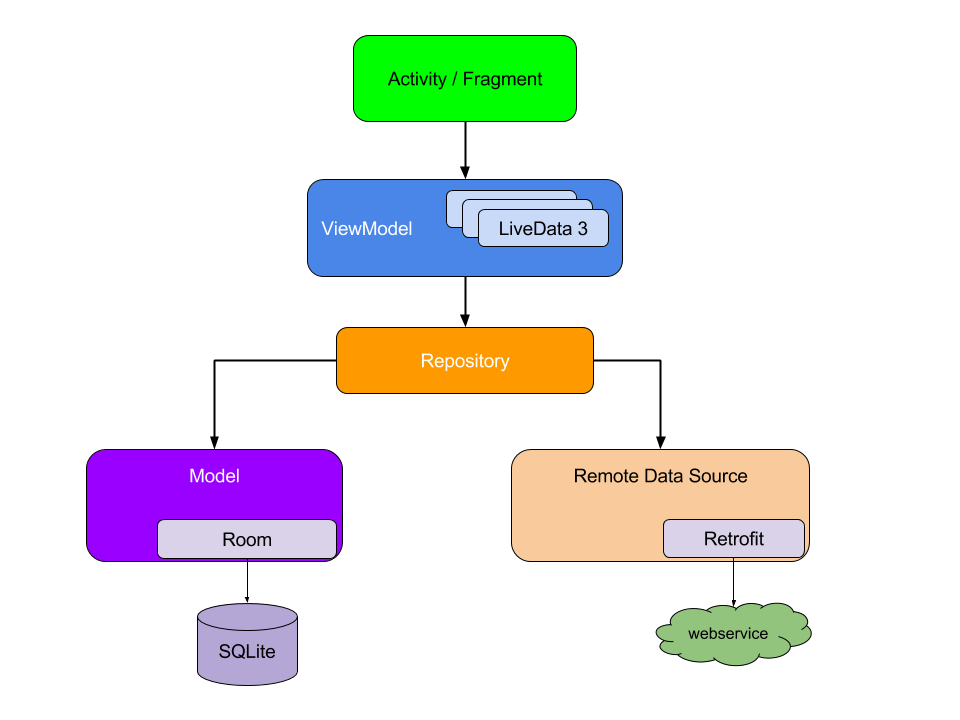
\includegraphics[width=0.7\textwidth]{pics/MVVM_repository.png}
%\caption{MVVM mit Data Layer  \cite{AndroidArchitectureComponents}}%
%\label{rrr}%
%\end{figure}
%die Aufteilung in View ("`Activity/Fragment"'), ViewModel, Model und Data Layer mit bestehendem Repository als Zugriffs-Abstraktion.
